\chapter{Peer discovery}
\label{cha:discovery}
This chapter discusses the design of the peer discovery mechanisms in NanoTorrent. These mechanisms enable peers to discover other peers downloading the same torrent, allowing them to connect with each other and exchange file data. NanoTorrent uses a hybrid approach consisting of two peer discovery mechanisms running side-by-side, allowing it to exploit locality while at the same time keeping distant nodes connected.

Section \ref{sec:discovery:tracker} describes the client-server approach using a centralized tracker. Section \ref{sec:discovery:local} discusses the local peer discovery mechanism using \gls{IPv6} local multicasts. Finally, section \ref{sec:discovery:conclusion} concludes with a discussion of the hybrid approach.

\section{Peer discovery with centralized tracker}
\label{sec:discovery:tracker}
One approach to implementing peer discovery is using a client-server architecture where membership information is provided by a central server known as the \emph{\gls{tracker}}. This tracker maintains the state of all peers in the \gls{swarm}, and peers can discover and be discovered by other peers by sending requests to obtain (parts of) this information.

\subsection{Requirements}
The \gls{tracker} is responsible for maintaining the \emph{\gls{swarm}} of each of its torrents, i.e. the list of \glspl{peer} for every tracked torrent. It must be notified when a peer wants to join the swarm to start downloading a torrent, and when it wants to leave after it finishes downloading and seeding the torrent. In order to deal with possible peer failures, messages from peers to the tracker are also treated as a `heartbeat' for that peer. The tracker keeps track of the timestamp of the last message from each peer and periodically removes peers who have not contacted the tracker for a long time. This helps to ensure that peers will discover active peers most of the time and will not try to connect with unreachable stale peers.

Peers should be able to discover other peers by contacting the tracker and receiving a list of other peers with whom to connect. Each peer is responsible for keeping the tracker up-to-date on its own participation state, such as when it joins or leaves the swarm. This allows the peer to be discovered by other peers when they contact the tracker themselves. In order to keep their heartbeat alive at the tracker, peers need to periodically contact the tracker to refresh their state as long as they're participating in the swarm.

\subsection{Torrent descriptor}
\label{sec:discovery:torrent-desc}
Before a file can be distributed to a set of nodes in the network, these nodes must have enough information to download and verify the whole file on their own. This information is contained in a \emph{\gls{torrent-desc}} which is generated upfront and needs to be made available at every node to start the file transfer.

The \gls{torrent-desc} is similar to the \emph{metainfo} in BitTorrent, but uses a denser structure than BitTorrent. This allows for a shorter descriptor file compared to BitTorrent's \texttt{.torrent} file, and faster parsing by nodes.

A \gls{torrent-desc} consists of the \gls{IP} address and port of the tracker, and the \gls{torrent-info} (further explained in \ref{sec:distrib:piece}. Like BitTorrent, trackers and nodes use the \gls{torrent-info-hash} calculated from the \gls{torrent-info} as an identifier for a torrent (see \ref{sec:related:bittorrent}). This way, a node only needs the torrent descriptor to locate the tracker and join the swarm corresponding to the correct torrent.

The distributor must generate the torrent descriptor and make it available to all destined nodes before starting file distribution. How the torrent descriptor is made available at a node, is out of the scope of the protocol.

\subsection{Protocol}
Peers communicate with the tracker through a request-reply protocol, (unimaginatively) named NanoTracker. This is a simple request/reply protocol over \gls{UDP}, where peers send an \emph{announce request} to the tracker, and the tracker responds with an \emph{announce reply}. Since the tracker can potentially track multiple swarms for multiple torrents, every message also includes the info hash of the torrent to identify the swarm. In theory, this allows a peer to join multiple swarms and download multiple torrents concurrently, although the current implementation supports only one concurrent torrent download.

The address of the tracker is included in the torrent descriptor, which must be available to every peer to participate in the torrent. A peer sends an announce request to this address over \gls{UDP}, including the event of the request and the maximum number of peers that it wants to receive in the reply. Since different clients may have different resource constraints, a client may want to request more peers from the tracker if it wants to connect with more peers simultaneously. The event indicates the reason for sending the request, and determines how the tracker should react to the request:
\begin{description}
\item[started] The peer wants to start downloading the torrent. The tracker should add the peer to the swarm, and allow it to be discovered by other peers.
\item[stopped] The peer has stopped downloading the torrent. The tracker should remove the peer to the swarm, so it will no longer be discoverable by other peers.
\item[refresh] The peer wants to refresh its participation in the swarm. The tracker should update the peer's heartbeat timestamp, ensuring that it stays discoverable for the near future.
\item[completed] The peer has finished downloading the torrent and is now seeding the torrent. The tracker could use this information for statistics, or for prioritizing the peer in the replies for other peers.
\end{description}

The tracker selects a number of other peers from the swarm, making sure it does not exceed the maximum number of peers requested by the peer. The tracker then constructs and sends back an announce reply, which contains a list of \gls{IPv6} addresses of the selected peers. The peer stores these addresses and can then start connecting and exchanging pieces with those peers as described in chapter \ref{cha:distribution}.

\subsection{Comparison with BitTorrent}
The design of the tracker protocol is heavily inspired by the \gls{UDP} Tracker protocol for BitTorrent \cite{bep15}, but is adapted to the needs of \glspl{WSN}.

\subsubsection{IP spoofing prevention}
BitTorrent tries to prevent peers from `spoofing' their \gls{IP} addresses, i.e. using a different address as the \gls{UDP} source address than their own. A malicious user could abuse the peers in a very popular torrent's swarm for a \gls{DDoS} by spoofing an announce request with the victim's IP address. Since the BitTorrent tracker stores the source \gls{IP} address of the announce request and announces it to other peers looking to discover peers in the swarm, these peers can be tricked into sending traffic to the uninterested victim.

To prevent \gls{IP} spoofing, a peer has to first send a connect request and receive a connection identifier in the tracker's connect reply. This identifier must then be passed in every announce request and validated by the tracker. This way, the peer has to `prove' it is using its own IP address by presenting information sent to the provided source address.

In the context of \glspl{WSN}, \gls{IP} spoofing is not really a concern. Therefore, there is no need for an initial connect request/reply step and peers can immediately send announce requests.

\subsubsection{Random peer ports}
In BitTorrent, peers choose a random \gls{TCP} port to listen for incoming connections from other peers for the peer-to-peer protocol \cite{bep3}. This allows multiple torrent downloads to run on different ports without interfering with each other. However, this also means that other peers need to know both the \gls{IP} address as well as the port number of a peer in order to set up a connection. Therefore, a peer includes its port number in the announce request, the tracker stores this port along with the rest of the peer's information and announce replies contain both the IP address and the port number for each peer.

For \glspl{WSN}, it is more convenient if all peers use a fixed port number for peer-to-peer communication. This allows local peer discovery (detailed in \ref{sec:discovery:local}) to use a single multicast address and a single port to reach all local peers. A disadvantage of this approach is that now all peer messages must include the torrent's info hash to identify the torrent, as the same port could be used by multiple torrents being downloaded by different nodes in the network.

\subsubsection{Download and upload statistics}
In BitTorrent, peers must provide information about the amount of bytes they have uploaded and downloaded, as well as how much data they still have left to download in order to complete the torrent download. This statistical information can be used by the tracker for example to implement more sophisticated peer selection algorithms for generating announce replies, to analyse the `health' of the torrent or simply to display on the tracker's website.

In the context of \glspl{WSN}, this information is not really needed and therefore not supported by the NanoTracker protocol.

\subsection{Conclusion}
By centralizing membership information at a single tracker, it becomes easier to analyse the state of the swarm. An operator of the \gls{WSN} can query the tracker at any time and retrieve information about which peers are currently connected. The tracker can detect when a peer stops sending periodic announce refreshes, and notify the operator of a potentially failed peer.

However, the need to periodically refresh the swarm membership state of every peer inevitably leads to additional network traffic. It could also create a bottleneck in the section of the network closest to the tracker, where all messages from all peers in the \gls{WSN} need to pass.

\section{Peer discovery with local multicast}
\label{sec:discovery:local}
In many \glspl{WSN}, nodes with similar tasks are often deployed closely together. Some networks consist of small clusters of similar nodes, or only consist of one node type altogether. In these deployments, peers need the same files as their immediate local neighbours, and can distribute files more efficiently through local broadcasts to all of their neighbours (see \ref{sec:distrib:multicast}).

To encourage peers exchanging pieces of the distributed file with their immediate neighbours, peers need to be able to discover neighbour nodes which are downloading the same torrent. The local peer discovery mechanism achieves this by periodically sending an announcement as a multicast to all immediate neighbours. If a peer receives such a local advertisement, it can try to connect with the originating peer.

\subsection{IPv6 link-local multicast}
\gls{IPv6} supports three addressing modes: unicast, anycast and multicast \cite{rfc4291}. A unicast address identifies a single \gls{IPv6} interface, and a packet sent to it is delivered only to that interface. An anycast address identifies one or more interfaces, but a packet sent to it is delivered to \emph{one} of those interfaces. A multicast address also identifies multiple interfaces, but packets are delivered to \emph{all} of those interfaces. This is a big improvement over \gls{IPv4}, which only defines unicast and broadcast addresses (with \emph{optional} multicast support).

Orthogonal to addressing modes are address scopes, which indicate in which part of the network a given address is valid. Global addresses are valid over the whole Internet, whereas link-local addresses are only valid in a single network.

\gls{IPv6} reserves some special multicast addresses to send messages to certain types of nodes in an address scope. For example, a multicast address can target all nodes, all routers or all \gls{DHCP} servers on the same link, network or organization.

\subsection{Protocol}
The local peer discovery protocol consists of periodically sending an announcement to all direct neighbours. This allows local peers listening to these announcements to discover new peers and in return set up connections with them.

For the purpose of discovering other peers in the immediate neighbourhood, NanoTorrent currently uses the \texttt{ff02::1} link-local all-nodes multicast address. This address works like a link-layer local broadcast address (e.g. the \gls{MAC} address \texttt{ff:ff:ff:ff:ff:ff}). All nodes already listen to incoming packets on this address, requiring no extra configuration.

Rather than adding another special-purpose message type for periodic announcements, NanoTorrent re-uses the \texttt{have} message which is already periodically exchanged between peers (discussed in more detail in \ref{sec:distrib:connection}). Peers use this when setting up a connection to a newly discovered peer, and to periodically inform connected peers of their download progress. Local peer discovery is implemented by also sending these periodic \texttt{have} messages to the link-local all-nodes multicast address. When a local peer receives any message from an unknown peer, it will try to set up a peer connection and (eventually) send back their own message. This reply allows the originating peer to set up its own connection with the discovered peer, resulting in a two-way connection where both peers can request pieces.

\begin{figure}
    \centering
    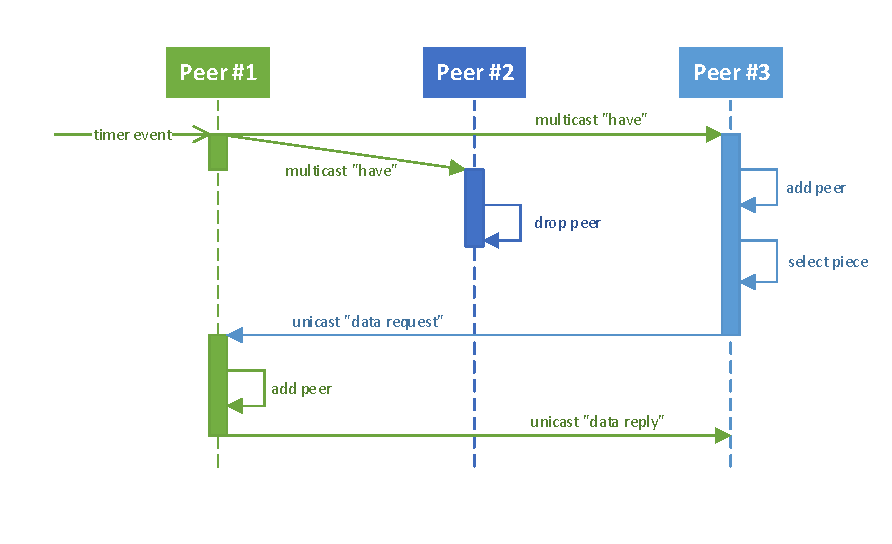
\includegraphics[width=\textwidth]{diagrams/local-peer-discovery.pdf}
    \caption[Sequence diagram of local peer discovery]{Sequence diagram of local peer discovery. The second peer has no more resources to add a connection for the first peer, and ignores the announcement. The third peer does add the new peer, and immediately requests a piece from the new peer. This allows the first peer to discover the third peer, add it and reply to the request.}
    \label{fig:discovery:local}
\end{figure}

Figure \ref{fig:discovery:local} shows a sequence diagram of a possible interaction between three neighbouring peers. The first peer sends its periodic announcement as a multicasted \texttt{have} message to all its neighbours. When they receive this message, they can choose to set up a connection with the peer if they have enough resources to do so and are downloading the same torrent. In this case, the third peer detects that the new peer has interesting pieces, and immediately sends a data request for a missing piece. The first peer receives this message from an unknown peer, which allows it to discover the third peer and add it to its own connections. It then dutifully responds to the request, and can start requesting pieces for itself. If the first peer did not have any pieces that are immediately interesting to the third peer, the third peer will later on send its own multicast announcement, so the first peer can eventually discover the third peer.

\subsection{Conclusion}
Local peer discovery can be added to NanoTorrent with minimal additional cost. For the wireless radio antenna, it doesn't matter whether a packet is destined to one or multiple nodes: all messages must be broadcasted anyway over the wireless medium. However, multicast packets do take more time for nodes to process, as they cannot short-circuit them like unicast messages. When a node receives a unicast packet destined to a different node, it can reject this as early as the link layer (using the destination \gls{MAC} address) or the network layer (using the destination \gls{IP} address). All-nodes multicast messages however always make it through to at least the transport layer, only rejecting the packet when the node is not acting as a NanoTorrent peer and therefore is not listening on the protocol's \gls{UDP} port.

By building on top of \gls{IPv6} multicast, local peer discovery can work on any \gls{IPv6}-compliant networking stack. Rather than going to a lower layer protocol such as \gls{RPL} \cite{rfc6550} for information about physical neighbours, NanoTorrent stays generic and independent of the underlying physical network infrastructure. This also allows it to re-use large parts of the existing protocol which is already designed for \gls{IPv6}.

\section{Conclusion}
\label{sec:discovery:conclusion}
Like in BitTorrent, the centralized tracker acts as a single source of (partial) truth about all active peers in a torrent's swarm. Every peer periodically announces itself to the tracker to keep its membership state alive, and in return received a list of other known peers in the swarm. Since this list is a random subset of the whole swarm, the chance of the \gls{P2P} network becoming partitioned is fairly low.

Local peer discovery ties in nicely with the peer wire protocol for the actual file distribution (see \ref{sec:distrib:connection}), and allows for a hybrid peer discovery solution. The tracker is still useful for ensuring that peers don't end up isolating themselves by only connecting to local peers, while local peers can efficiently propagate newly retrieved pieces to all of their immediate neighbours at once (see \ref{sec:distrib:multicast}).
